\documentclass[serif,envcountsect,table,t]{beamer}%, handout
\usepackage{amsmath, animate, hyperref, subcaption, tikz, multirow}
\usetheme{CambridgeUS}
\usecolortheme{wolverine}
% \usecolortheme{orchid}
\setbeamertemplate{navigation symbols}{}
\graphicspath{{../figures/}}
\addtobeamertemplate{frametitle}{}{\vspace{-3mm}} % reduce top space
%%%%----------------------------------------------------------
\begin{document}
\title[Bias and Sampling]{Pre College Summer - Data Science\\
Bias in Data Collection}
\author[Bar, Wang]{Haim Bar, HaiYing Wang}
\date[]{}
\institute[UConn]{\normalsize University of Connecticut}
%%%% -------------------------------------------------
\begin{frame}[noframenumbering] \titlepage \end{frame}
%%%% ----------------------------------------------------------
\begin{frame}{Representative sample}
  \begin{itemize}
  \item In data science, a population is the entire set of subjects that we
are interested in studying.
\item A sample is a subset of a population.
\item A
representative sample reflects the patterns in the population.
\item This is important because we want to use the
 sample to obtain conclusions on the population.
  \end{itemize}
    \begin{center}\-\\[-6mm]
      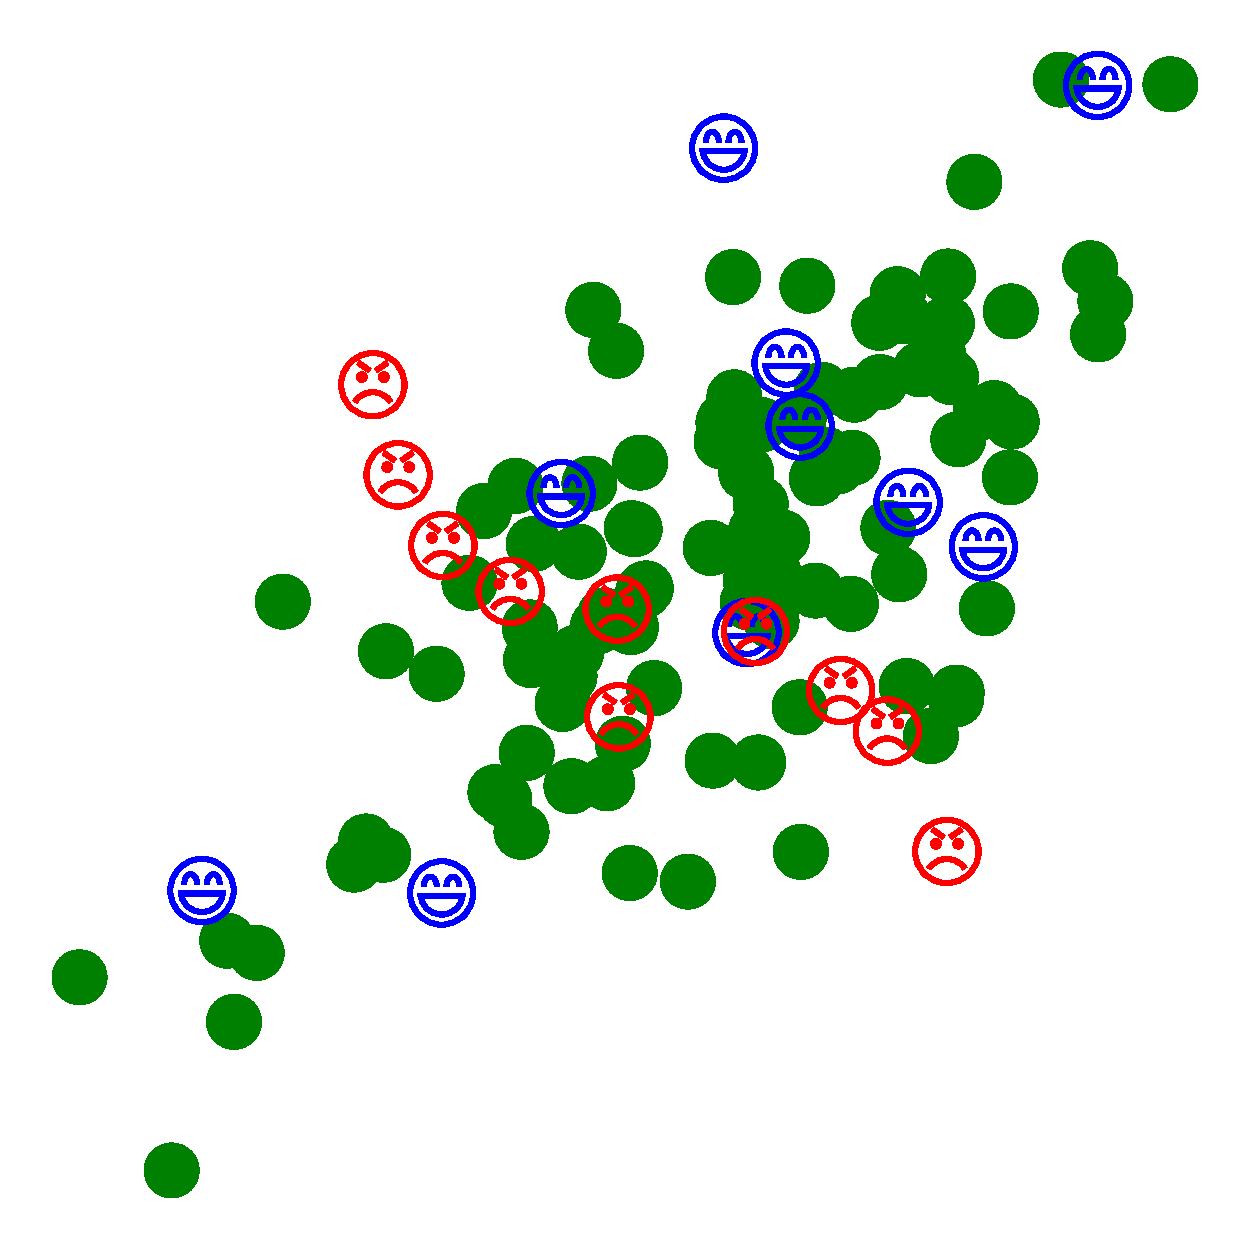
\includegraphics[width=0.5\textwidth]{GoodBadSamples.pdf}
  \end{center}
\end{frame}
%%%% ----------------------------------------------------------
\begin{frame}{Representative sample}
\begin{figure}
  \centering
    \begin{subfigure}{0.32\textwidth}
      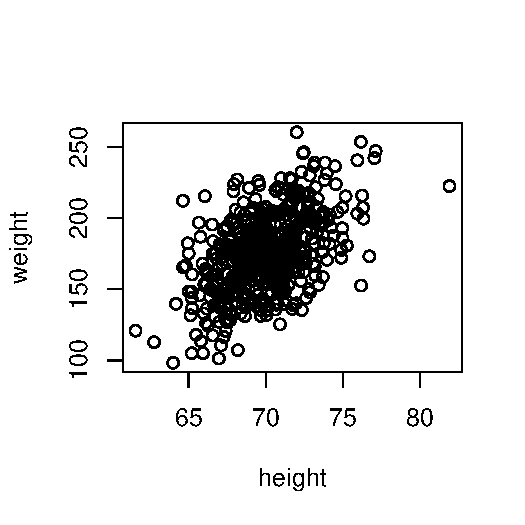
\includegraphics[width=\textwidth]{population.pdf}
      \caption{Population}
    \end{subfigure}
  \begin{subfigure}{0.32\textwidth}
      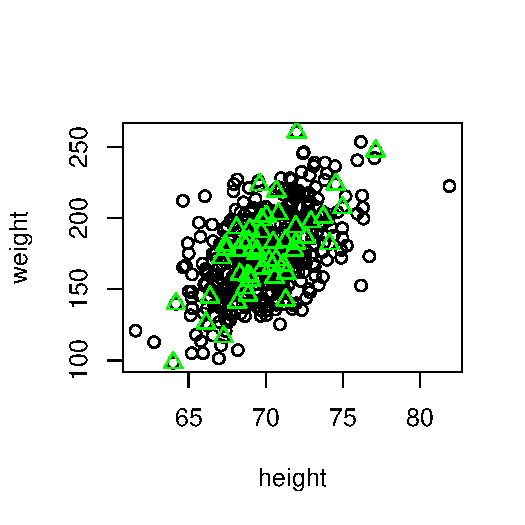
\includegraphics[width=\textwidth]{representSample.pdf}
      \caption{Representative sample}
  \end{subfigure}
  \begin{subfigure}{0.32\textwidth}
      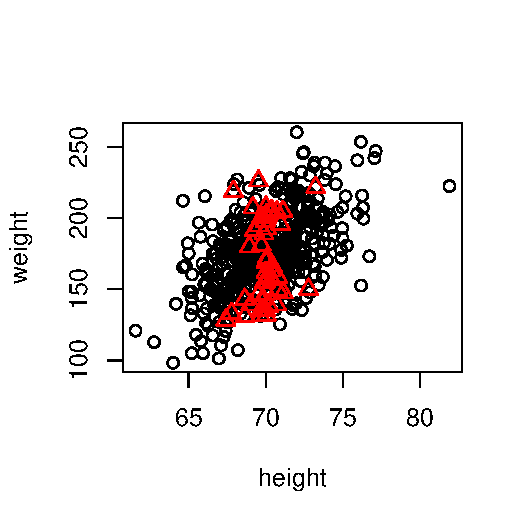
\includegraphics[width=\textwidth]{biasedSample.pdf}
      \caption{Biased sample}
  \end{subfigure}
  \caption{An illustrative of representative sample}
  \label{fig:representativesample}
\end{figure}
\end{frame}
%%%% ----------------------------------------------------------
\begin{frame}{Simpson's Paradox}
  Tanya and Sonya are two freshmen basketball players in college.
  \begin{enumerate}
  \item In the first three games of the season, Tanya had 11 free throws of
    which she made 5, and Sonya went 7 times and made 3 of the free throws.  If
    at the end of game three the coach want to pick the player with the better
    chance of making free throws, who should she choose?
    % Tanya's probability based on the first three games is $5/11 = .455$, while
    % Sonya's is $3/7 = .429$, so if the coach picks Tanya the team has a better
    % chance from the free throws line.
    \pause
  \item During the next three games, Tanya got 9 free throws and made 6, and
    Sonya got 14 free throws and made 9. Which player the coach will chose as
    the better free-throw shooter based on the last 3 games?
    \pause
  \item Which player the coach will chose as the better free-throw shooter based
    on all the six games?
    % choose Tanya's chances are $6/9 = .667$, while Sonya's are $9/14 =
    % .643$. So once again, the coach picks the player with the better chances,
    % and based on the last three games, it is Tonya once again.

    % Again, at the end of game six has to However, if we combine the results
    % from all six games we see that Tanya went to the line 11+9=20 times and
    % made 11 of the free throws, and Sonya got 7+14=21 free throws and made
    % 3+9=12. So, if we combine the results from all six games Tonya's
    % percentage from the free throw line is 55\%, while Sonya's is 57.1\%, so
    % based on the cumulative information Sonya should be the coach's pick!
  \end{enumerate}
\end{frame}
%%%% ----------------------------------------------------------
% \begin{frame}{Simpson's Paradox}
%   \begin{enumerate}
%   \item A black urn contains 5 red and 6 green balls, and a white urn contains 3
%     red and 4 green balls. You are allowed to choose an urn and then choose a
%     ball at random from the urn. If you choose a red ball, you get a
%     prize. Which urn should you choose to draw from?
% \pause
% % \begin{itemize}
% % \item If you draw from the black urn, the probability of choosing a
% %   red ball is $5/11 = .455$.
% % \item If you choose to draw from the white urn, the probability of
% %   choosing a red ball is $3/7 = .429$.
% % \end{itemize}
% % You should choose to draw from the black urn.
%   \item Now consider another game in which a second black urn has 6 red and 3
%     green balls, and a second white urn has 9 red and 5 green balls.  Which urn
%     should you choose to draw from?
%     \pause
%   \item In the final game, the contents of the second black urn are added to the
%     first black urn, and the contents of the second white urn are added to the
%     first white urn. Again, you can choose which urn to draw from. Which should
%     you choose?
%   \end{enumerate}
% \end{frame}
% %%%% ----------------------------------------------------------
% \begin{frame}{Simpson's Paradox}
% Now consider another game in which a second black urn has 6 red and
% 3 green balls, and a second white urn has 9 red and 5 green balls.
% % \pause
% % \begin{itemize}
% % \item If you draw from the black urn, the probability of a red ball is
% %   $6/9 = .667$.
% % \item If you choose to draw from the white urn, the probability if
% %   $9/14 = .643$.
% % \end{itemize}
% Again you should choose to draw from the black urn.\\[7mm]
% In the final game, the contents of the second black urn are added to
% the first black urn, and the contents of the second white urn are
% added to the first white urn. Again, you can choose which urn to draw
% from. Which should you choose?
% \end{frame}
%%%%----------------------------------------------------------
\begin{frame}{UC Berkeley gender bias}
A famous example of Simpson's
paradox is a study of gender bias among graduate school admissions to
University of California, Berkeley. In 1973 UC Berkeley was sued for
sex-discrimination. Here are the overall numbers for the six largest
departments in fall admission of 1973.

\begin{center}
  \begin{tabular}{crrcrr}\hline
    \multicolumn{3}{c}{Men} & \multicolumn{3}{c}{Women} \\\hline
    Applicants & \multicolumn{2}{c}{Admitted} & Applicants
                                      & \multicolumn{2}{c}{Admitted} \\\hline
    2691 & 1198 & ({\bf 44.5}\%) & 1835 & 557 & (30.4\%) \\\hline
  \end{tabular}
\end{center}
This table shows that men were more likely than women to be admitted,
and the difference was so significant. Let's see which departments
were mainly responsible for this gender bias. To do this we broke open
the data according to each departments.
\end{frame}
%%%%----------------------------------------------------------
\begin{frame}{UC Berkeley gender bias}

\begin{center}
  % \centering
\begin{tabular}{ccrrcrr}\hline
  & \multicolumn{3}{c}{Men}  & \multicolumn{3}{c}{Women} \\\cline{2-7}
  Department & Applicants  & \multicolumn{2}{c}{Admitted} & Applicants
                           & \multicolumn{2}{c}{Admitted} \\\hline
A & 825 & 512& (62\%) & 108 & 89 &(82\%)  \\ 
B & 560 & 353& (63\%) & 25  & 17 &(68\%)  \\
C & 325 & 120& (37\%) & 593 & 202& (34\%) \\
D & 417 & 138& (33\%) & 375 & 131& (35\%) \\
E & 191 & 53 & (28\%) & 393 & 94 &(24\%)  \\
F & 373 & 22 & (6\%) & 341 & 24 &(7\%)  \\\hline
\end{tabular}
\end{center}

Things get strange after we divide the data according different
departments. For the six departments, four of them accepted women more
than men. The reason is that women
tended to apply to more competitive departments with low admission
rates even among qualified applicants, whereas men tended to apply to
less competitive departments with high admission rates among the
qualified applicants.
\end{frame}
%%%% -------------------------------------------------
\begin{frame}{Are these impressions real facts?}
  \begin{itemize}
  \item Hollywood ruins good books.
    \begin{itemize}
    \item \href{https://www.yardbarker.com/entertainment/articles/popular_books_that_were_made_into_terrible_movies/s1__29971472}{Popular books that were made into terrible movies}
    \item \href{https://www.listchallenges.com/great-movies-based-on-bad-books}{Great Movies Based on Bad Books} 
    % \item \href{https://www.tckpublishing.com/best-movies-based-on-books/}{25 Best Movies Based on Books}
    \end{itemize}
  \item Handsome men are such jerks.
  \item Pretty girls are mean.
  \item More talented people are less attractive.
  \item Smarter students spend less time on studying. 
  \item % The list can go on forever
    ...
  \end{itemize}
\end{frame}
%%%%----------------------------------------------------------
\begin{frame}{Berkson's bias: stumps display example}
  \begin{itemize}[<+->]
  \item Suppose you have 1000 postage stamps: 300 are pretty, 100 are rare, and 30 are both pretty and rare. Is a rare stamp more likely to be pretty?
  \item Now you want to show some of your stamps to your friends, you probably want to show them the pretty ones and the rare ones. 
  \item Lets say you only show the 370 stamps which are either pretty or rare to your friends. Based on what your friends observed, will they conclude that a rare stamp more likely to be pretty?
  \end{itemize}
\end{frame}
%%%%----------------------------------------------------------
\begin{frame}
  During World War II, aircraft that had returned from missions were examined and  the most-hit areas of the plane are given in the following figure. Which areas should the army add armor to increase the survivorship of the planes?
  \begin{center}\-\\[-6mm]
      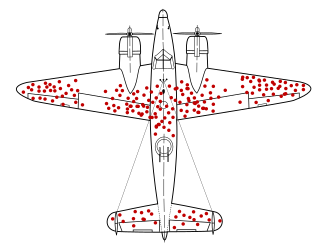
\includegraphics[width=0.75\textwidth]{Survivorship-bias.png}
  \end{center}
\end{frame}
%%%%----------------------------------------------------------
\begin{frame}{Survival Bias}
  \begin{itemize} % [<+->]
  \item A direct intuition may suggest to reinforce areas with the most bullet holes. However, this is not a wise decision. Why? 
  \item The data were collected from the aircraft that had survived their missions so they are biased. 
  \item Planes that had been shot down or otherwise lost had not been counted. 
  \item The bullet holes in the returning aircraft represented areas where a plane could take damage and still fly well enough to return safely. 
  \item Thus, it is the areas where the returning aircraft were unscathed that need additional armor.
  \end{itemize}
\end{frame}
%%%%----------------------------------------------------------
\begin{frame}{The 1936 Literary Digest Poll}
  \begin{itemize}
  \item For the 1936 presidential election, the Literary Digest predicted that Alfred Landon would get 57\% of the vote against Franklin D. Roosevelt's 43\%, while the actual results were 62\% for Roosevelt against 38\% for Landon.
  \item The Literary Digest poll was one of the largest and most expensive polls with a sample size of around 2.4 million people!
  \item At the same time, George Gallup was able to predict a victory for Roosevelt using a much smaller sample of about 50,000 people.
  \item Literary Digest's sampling method: Based on every telephone directory in the United States, lists of magazine subscribers, rosters of clubs and associations, and other sources, a mailing list of about 10 million names was created. Every name on this list was mailed a mock ballot and asked to return the marked ballot to the magazine.
  \end{itemize}
  
%   The presidential election of 1936 pitted Alfred Landon, the Republican governor of Kansas, against the incumbent President, Franklin D. Roosevelt. The year 1936 marked the end of the Great Depression, and economic issues such as unemployment and government spending were the dominant themes of the campaign. The Literary Digest was one of the most respected magazines of the time and had a history of accurately predicting the winners of presidential elections that dated back to 1916. For the 1936 election, the Literary Digest prediction was that Landon would get 57\% of the vote against Roosevelt's 43\% (these are the statistics that the poll measured). The actual results of the election were 62\% for Roosevelt against 38\% for Landon (these were the parameters the poll was trying to measure). The sampling error in the Literary Digest poll was a whopping 19\%, the largest ever in a major public opinion poll. Practically all of the sampling error was the result of sample bias.

% The irony of the situation was that the Literary Digest poll was also one of the largest and most expensive polls ever conducted, with a sample size of around 2.4 million people! At the same time the Literary Digest was making its fateful mistake, George Gallup was able to predict a victory for Roosevelt using a much smaller sample of about 50,000 people.
\end{frame}
%%%%----------------------------------------------------------
\begin{frame}{Common sources of biases}
\begin{itemize}
\item Observation time interval: Early termination of a trial at a time when its results support the desired conclusion.
\item Data partition: divide data with knowledge of the contents of the partitions. 
\item Confirmation bias: to search for, interpret, favor, and recall information in a way that confirms or supports one's prior beliefs or values. A famous example is cherry picking. The picker would be expected to select only the ripest and healthiest fruits. An observer who sees only the selected fruit may thus wrongly conclude that most, or even all, of the tree's fruit is in a likewise good condition.
\item Self-selection bias or a volunteer bias.  % in studies offer further threats to the validity of a study as these participants may have intrinsically different characteristics from the target population of the study. Studies have shown that volunteers tend to come from a higher social standing than from a lower socio-economic background.[20] Further, to this another study shows that women are more probable to volunteer for studies than males. Volunteer bias is evident throughout the study life-cycle, from recruitment to follow-ups. More generally speaking volunteer response can be put down to individual altruism, a desire for approval, personal relation to the study topic and other reasons.[20][14] As with most instances mitigation in the case of volunteer bias is an increased sample size.[c
\item Nonresponse bias: It is often related to sensitive questions.
\end{itemize}
\end{frame}
%%%% ----------------------------------------------------------
\begin{frame}{Common sources of biases}
\begin{itemize}
\item Rejection of bad data on (1) arbitrary grounds, instead of according to previously stated criteria or (2) discarding ``outliers'' on statistical grounds that fail to take into account important information that could be derived from ``wild'' observations.
\item Length time bias: It often occurs in cancer screening studies. Compared with fast-growing tumors, slow-growing tumors has a longer period of time during which the cancer is in the body but not large enough to cause symptoms. Thus if the same number of slow-growing and fast-growing tumors appear in a year, the screening test detects more slow-growers than fast-growers. If the slow growing tumors are less likely to be fatal than the fast growers, the people whose cancer is detected by screening do better, on average, than the people whose tumors are detected from symptoms. This may give the impression that detecting cancers by screening causes cancers to be less dangerous.  % even if less dangerous cancers are simply more likely to be detected by screening.[1]
\end{itemize}
\end{frame}
%%%%----------------------------------------------------------
\begin{frame}{Some basic sampling designs}
  \begin{itemize}
  \item Simple Random Sampling: Every elements in the target population have equal chances to be selection. Samples are selected strictly by chance. It is probably the most effective method to prevent sampling bias. A disadvantage is the uncertainty may be large.
  \item Stratified Sampling: Divide members of the population into homogeneous subgroups and then use simple random sampling for each subgroups. It helps to reduce the uncertainty. Need to be careful of potential biases.
  \item Weighted Sampling: Let more informative elements have higher chances to be selected. It may increase the estimation efficiency, but the resulting sample may be biased so need special way of estimation.
  \end{itemize}
\end{frame}
%%%%----------------------------------------------------------
\begin{frame}{Different sampling approaches}
  \begin{itemize}
  \item Sampling with replacement: An element may be included in a sample more than once. It is possible to have replicates in the sample.
  \item Sampling without replacement: An element can be included in a sample at most once. There is no replicates in the sample.
  \item Poisson sampling: determines if each element of the population is selected in the sample independently. The sample size is random.
  \item Between Sampling with replacement and without replacement, which is more efficient?
  \end{itemize}
\end{frame}
% %%%%----------------------------------------------------------
% \begin{frame}{Numerical comparisons}
%   \begin{itemize}
%   \item To simulation hosehold incomes, generate a population $P$ of size $N$
%     from a Poisson distribution. 
%     % $P\sim\chi^2$ distribution with degrees of freedom one.
%   \item Take samples of size $n$ from $P$ to estimate the population mean, say $\mu$, using simple random sampling both with and without replacement. Compare their efficiency.
%   \item Assume another variable $A=P+Unif(0,2)$ is available to define informative sampling weights. Evaluate the efficiency of weighted sampling both with and without replacement. 
%   \end{itemize}
% \end{frame}
% % %%%%----------------------------------------------------------
% % \begin{frame}{}
% % \end{frame}
% % %%%% ----------------------------------------------------------
\end{document}
